% Chapter Template

\chapter{Background} % Main chapter title

\label{Chapter2} % Change X to a consecutive number; for referencing this chapter elsewhere, use \ref{ChapterX}

\lhead{Chapter 2. \emph{Background}} % Change X to a consecutive number; this is for the header on each page - perhaps a shortened title

This chapter introduces the concepts and techniques that are relevant throughout this thesis. First, the concept of similarity search, especially the two software suite FASTA and BLAST would open our chapter. And then, we would introduce various contemporary concepts in bioinformatics and bioinformatics-related infrastructure such as UniProt and MEDLINE. Additionally, we would introduce the concept of named entity recognition (NER) within the field of Natural Language Processing and how it would be relevant for us. Finally we would see how our project relates to previous works in similar topics and how it would improve, provide alternative or give additional insight to them.

%----------------------------------------------------------------------------------------
%	SECTION 1
%----------------------------------------------------------------------------------------

\section{FASTA and BLAST}

As the title of this thesis already conveyed, the main idea of this project is to bridge the accessibility and knowledge gap between sequence and the main source of knowledge and reference of previous discoveries -- a vast corpora of publications in natural sciences -- through a modern search engine. Given a sequence of amino acids, it would be impossible for a human to directly identify directly the protein, let alone the characteristics and the functions and the characteristics of the protein.

Several attempts on bridging one component of the gap, specifically between sequence and other known sequences, was done in eighties and earlier nineties. In 1981, Smith and Walterman published the algorithm computing complete local sequence alignment, which was further improved by Gotoh in 1982 \citep{gotoh1982improved} and Altschul (Altschul and Erickson, 1986 \citep{altschul1986optimal}). This was however deemed too slow, especially if used for the purpose of one-against-all search, which was heavily (and still is) used for sequence-based knowledge discovery in biomedical research.

In 1985, Lipman and Pearson published the first paper mentioning the DNA and protein sequence alignment program FASTA \citep{Lipman85}. During the first publication, FASTA was designed and intended to search for similar protein sequences. It takes a sequence of amino acids and searches against entries within a corresponding database by using local sequence alignment to find similar sequences. In general, FASTA takes four steps in computing three scores that characterize sequence similarity \citep{Pearson19905}:

\begin{enumerate}
\item Finding identify regions with high density of sequence identities and pair identities between two sequences. FASTA achieved a fast computation in this step by using a look up table, a map that describes for each character where it appears within sequence. In conjunction with the lookup table, FASTA also uses the diagonal method to find 
all regions of similarity between the two sequences, counting matches and penalizing for intervening mismatches. This diagonal could be visually seen in two sequence alignment as series of matches ('dots') in match matrix between two sequences.

\item Rescanning of the 10 regions with highest sequence identities using PAM250 matrix. PAM250 matrix refers to assumed point accepted mutation (PAM) matrix after 250 mutations, which is basically the 250-th power of initial PAM matrix. The probability of each entry within PAM matrix was acquired from analysis of phylogenetic trees (Dayhoff, 1978 \citep{Dayhoff1978model}).

\item Annealing of both ends of alignment and calculating similarity score is the sum of the joined initial regions minus a penalty (usually 20) for each gap \citep{Pearson19905}.

\item Construction of optimal alignment using Needleman-Wunsch Algorthm \citep{needleman1970general} on the best matching region. The program would then return the similarity score of this alignment along with the best score from step 2 and 3.
\end{enumerate}

In 1988, Pearson and Lipman improved the software by adding support and improvement, among others, for nucleic acid similarity search, translated nucleic acid search \citep{PearsonLipman88}. This allowed researchers to do trans-domain search between nucleic and amino acids.

Further down the road, in 1990, Altschul et al. published the Basic Alignment Research Too \citep{Altschul90}, better known in its acronym as BLAST. The algorithm, like FASTA, is based on heuristics search and is structured in similar manner to BLAST. BLAST takes a sequence to search for and a sequence or a set of sequences to search against. In modern usage, the set of sequences is provided by some database. The algorithm would then run in following main steps \citep{mount2001bioinformatics}:

\begin{enumerate}
\item Removal of low complexity regions or sequence repeats from query sequence. Low complexity refers to sequence with few elements.
\item Creation of k-gram sequences from query sequence.
\item For each word from step 2, listing of possible matching words and selection of high scoring words. Matching words are the all possible combinations of words with same length as the k-gram word. For each possible word a score is calculated, which is based on substitution matrix. The best scoring words are then passed onto next step. This differs from FASTA, which focuses more on common words in database.
\item Organization of remaining high scoring words into efficient search three. Both step 3 and 4 would be repeated for each word from step 2.
\item Scanning of database for exact matches with remaining high-scoring words.
\item Extension of database match to high-scoring-segment pair (HSP). This is done by annealing both ends of match until the matching score begins to decrease.
\item Listing of all HSPs that are significant enough.
\item Evaluation of statistical significance of the HSPs. BLAST models statistical significance using Gumbel extreme value distribution \citep{gumbel1954statistical}, in which the probability of observing score $S$ higher than equal to $x$ is defined as $$P(S \leq x) = 1 - exp(-e^{- \lambda (x - \mu)})$$ with $$\mu = log(Km'n')/t$$ The parameters $\mu$ and $K$ are fitted from the distribution of results from high scoring pairs. m' and n' are effective length of the query and database sequences.
\item Make two or more HSP regions into one alignment. In a given hit sequence from database, the algorithm would attempt merging the regions into one had the score of combined region is larger than individual score.
\item Computation of sequence alignments using Smith-Walterman Algorithm \citep{smith1981identification}.
\end{enumerate}

Nowadays, both FASTA and BLAST were distributed not only locally but also online by various providers such as National Center of Biotechnology Information (NCBI)\footnote{\href{http://blast.ncbi.nlm.nih.gov/Blast.cgi}{\texttt{http://blast.ncbi.nlm.nih.gov/Blast.cgi}}, accessed 8/19/2015} and European Bioinformatics Institute (EBI)\footnote{\href{http://www.ebi.ac.uk/Tools/sss/wublast/}{\texttt{http://www.ebi.ac.uk/Tools/sss/wublast/}}, accessed 8/19/2015} \footnote{\href{http://www.ebi.ac.uk/Tools/sss/fasta/}{\texttt{http://www.ebi.ac.uk/Tools/sss/fasta/}}, accessed 8/19/2015}.

%----------------------------------------------------------------------------------------
%	SECTION 2
%----------------------------------------------------------------------------------------

\section{UniProt}

UniProt (\textit{Universal Protein Resource} \citep{uniprot2008universal}) is platform containing various high quality databases that are essential in bioinformatics research. A joint venture between European Bioinformatics Institute (EBI), Swiss Bioinformatics Institute (SBI) and Protein Information Resources (PIR), it provide four main sets of database: 

\begin{itemize}
\item \textbf{UniProt KnowledgeBase (UniProtKB)}, containing protein database. Our database of interest in this system, there are two main constituents of UniProtKB: the manually annotated, reviewed UniProtKB/SwissProt and automatically entried, unreviewed  UniProtKB/TrEMBL. Currently, there are 549,008 reviewed and 50,011,027 unreviewed protein sequences within the UniProtkB environment\footnote{\href{http://www.uniprot.org/}{\texttt{http://www.uniprot.org/}}, accessed 8/19/2015}. We consider the current ever widening over-representation of unreviewed proteins within the KnowledgeBase be a potential challange in our project going forward.

\item \textbf{UniProt Archieve (UniParc)}, a comprehensive and non-redundant database containing all protein sequences from publicly available protein sequence database \citep{leinonen2004uniprot}. It achieved redundancy by searching for each sequence only once. Multiple matching sequences from various databases would then be merged into one UniParc entry.

\item \textbf{UniProt Reference Cluster (UniRef)}, a set of three databases of clustered sets of proteins. The databases house clusters sets of proteins with 50\% (UniRef50), 80\% (UniRef80) and 90\% (UniRef90) sequence similarity \citep{suzek2007uniref}.

\item \textbf{UniProt Metagenomics and Environmental Data (UniMES)}, a repository for metagenomics and metagenomics sequences. UniMES was initially developed to address issues arising from sequences that are obtained from non-cultured or currently unknown organisms, which are sometimes used in metagenomics studies \citep{uniprot2008universal}. The data from UniMES is included in UniParc but not UniProtKB.
\end{itemize}

Each entry within UniProt main databases possesses a unique identifier. For UniProtKB, every entry within the database is associated with both UniProtKB accession number (UniProtKB-AC) and UniProtKB identifier (UniProtKB-ID). In this project, we use not only UniProtKB-ID as the identifier of choice when it comes to UniProt, but also as our main project identifier protein names. That is, a protein is always identified with UniProtKB-ID within our search engine, each annotation of mentions in text would be represented as UniPritKB-ID and our BLAST search will also return UniProtKB-ID. Consequently, this limits our search and indexing space within the scope that is already defined by UniProtKB. However, considering proteins that are of interest to the scientist are almost always already indexed by UniProtKB\citep{leinonen2004uniprot}, we don't really see this issue as potential problem.

%----------------------------------------------------------------------------------------
%	SECTION 3
%----------------------------------------------------------------------------------------

\section{MEDLINE}

MEDLINE contains journal citations and abstracts for biomedical literature around the world \citep{MEDLINE}. It is maintained by U.S. National Library of Medicine and currently houses over 24 millions of journal abstracts and the numbers keep growing along the new publications, which currently clocks at 7 per cent growth per year, which corresponds to over one million new articles in the last years \citep{larsen2010rate}. In MEDLINE environment alone, it adds between 2,000 - 4,000 references each day \citep{MEDLINE}. Last year alone, it added 750,000 new references into its repository \citep{MEDLINE}. The subject of journals that are indexed by MEDLINE ranges from life sciences, behavioral sciences, chemical science and bioengineering. While the overwhelming majority of the references indexed are journal articles, there are several newspaper and magazine entries that are deemed useful as reference in biomedical research. Ninety five percent of the articles are written in English and 84\% have English abstracts written by the authors of the articles.

For most part, a researcher could access MEDLINE through PubMed\footnote{\href{http://www.ncbi.nlm.nih.gov/pubmed}{\texttt{http://www.ncbi.nlm.nih.gov/pubmed}}, accessed 19/08/2015} \citep{MELDINEWeb}. This already covers about about 90\% of its indexed abstracts. For complete access, it offers leasing mechanism. It distributes daily the new references in XML format via FTP protocol. We use this leasing mechanism in our project for intial references collection and daily updates.

%----------------------------------------------------------------------------------------
%	SECTION 4
%----------------------------------------------------------------------------------------

\section{Natural Language Processing}

The rapid development in sequence similarity search coupled with explosion of genome-wide sequencing, which was even more augmented by the advent of post-Sanger and -- recently -- New Generation Sequencing (NGS), means that the problem of identifying sequence is more or less explained. There is however one part that is missing from our picture: how to get the information on how the sequence was mentioned in previous publications?

Come Natural Language Processing (NLP). Natural Language Processing is a interdisciplinary field that deals with the interaction between computer and human languages (hence the natural language). The aspects of natural languages such as named entities recognition (NER) \citep{nadeau2007survey}, morphological segmentation \citep{meyer1990morphological}, speech recognition and analysis  \citep{rabiner1993fundamentals} fall into the auspice of natural language processing. The methods used in natural language processing is mostly statistical-based \citep{manning1999foundations} and some of the methods have been known to be used in other fields such as Conditional Random Fields \citep{sutton2006introduction} and its special case Hidden Markov Chain, which is one of the more commonly used methods in bioinformatics (e.g. Salzberg, et al. \citep{salzberg1998microbial} and Burge, et al. \citep{burge1998modeling}).

In this thesis we would make use of one aspect of natural language processing: named entity recognition (NER).


%-----------------------------------
%	SUBSECTION 4.1
%-----------------------------------


\subsection{Named Entity Recognition}

\label{ssec:NERC2}

The term named entity recognition was first coined at the Sixth Message Understanding Conference (MUC-6) in 1996 \citep{nadeau2007survey} \citep{grishman1996message}. The problem statement of named entity recognition roughly goes as follow:

\begin{center}
\textit{Given an input text, locate and classify elements of text according to defined categories of entity (a Named Entity)}
\end{center}

The pre-defined set of categories range from unique identifier such as name and location to expression of times and numeric values such as date and percent expression \citep{nadeau2007survey}. To take an example, consider the first paragraph of following recent article from the Wall Street Journal\footnote{\texttt{\href{http://www.wsj.com/articles/uber-valued-at-more-than-50-billion-1438367457}{http://www.wsj.com/articles/uber-valued-at-more-than-50-billion-1438367457}}, accessed 8/19/2015}:

\begin{displayquote}
{\Large Uber Valued at More Than \$50 Billion}


\textbf{Ride-sharing app, which just closed a funding round, reaches mark faster than Facebook}

Uber Technologies Inc. has completed a new round of funding that values the five-year-old ride-hailing company at close to \$51 billion, according to people familiar with the matter, equaling Facebook Inc.’s record for a private, venture-backed startup.

\end{displayquote}

A named entity recognition program trained for company names and monetary values would identify and tag following annotations from the text:

\begin{displayquote}
{\Large \textbf{Uber} \texttt{(company)} Valued at More Than  \textbf{\$50 Billion } \texttt{(monetary\_value)}}


\textbf{Ride-sharing app, which just closed a funding round, reaches mark faster than \textbf{Facebook} \texttt{(company)}}

\textbf{Uber Technologies Inc.} has completed a new round of funding that values the five-year-old ride-hailing company at close to \textbf{\$51 billion} \texttt{(monetary\_value)}, according to people familiar with the matter, equaling \textbf{Facebook Inc.} \texttt{(company)}’s record for a private, venture-backed startup.

\end{displayquote}

Here we see how various formats of company names could be tagged in this hypothetical case. Indeed, a good named-entity recognition tagger should be able to perform exactly this kind of task.

There are various ways of implementing Named Entity Recognition (NER), all ranging from supervised, semi-supervised to unsupervised learning \citep{nadeau2007survey}. Nowadays, most NER relies on supervised learning methods \citep{nadeau2007survey} such as Hidden Markov Model (HMM) \citep{bikel1997nymble}, Decission Trees \citep{sekine1998decision}, Maximum Entropy Model \citep{borthwick1998exploiting}, Support
Vector Machines (SVM) \citep{asahara2003japanese} and Conditional Random Fields (CRF)\citep{mccallum2003early}, which is a discriminative generalization of HMM\citep{lafferty2001conditional}.

In this project, we attempted on two distinct NER implementations: \textbf{DNorm} in the earlier phase and non-publicly available NER tagger given to us by Lars Juhl Jensen at University of Copenhagen (which would for our convenience would be called \textbf{STRING Tagger} or \textbf{(PubSeq) NER Tagger} from now on) later on. DNorm (Leaman and Lu, 2013 \citep{leaman2013dnorm}) is a NER designed to tag and normalize disease names within PubMed abstract. Given a PubMed abstract text, it tags the disease entities within text and normalize said entities into standardized form (in this case, MEDIC concepts \citep{davis2012medic}). The tagging component of DNorm is based on BANNER, which in turn is a CRF-based NER tagger \citep{leaman2008banner}. To normalize the entities, the program utilizes pairwise approach of Learning to Rank \citep{liu2009learning} (see, for example, Joachims 2002 \citep{joachims2002optimizing}, which is used to rank the results of web search). The idea of ranking as a method of normalization could indeed be explained analogously in light of search engine itself, given a tagged string $s$, a set of standardized entity names $N$ and a scoring function $M(s, n) \in R$, we would like to find out to which standardized name this string maps best to.

\begin{figure}[htbp]
  \centering
    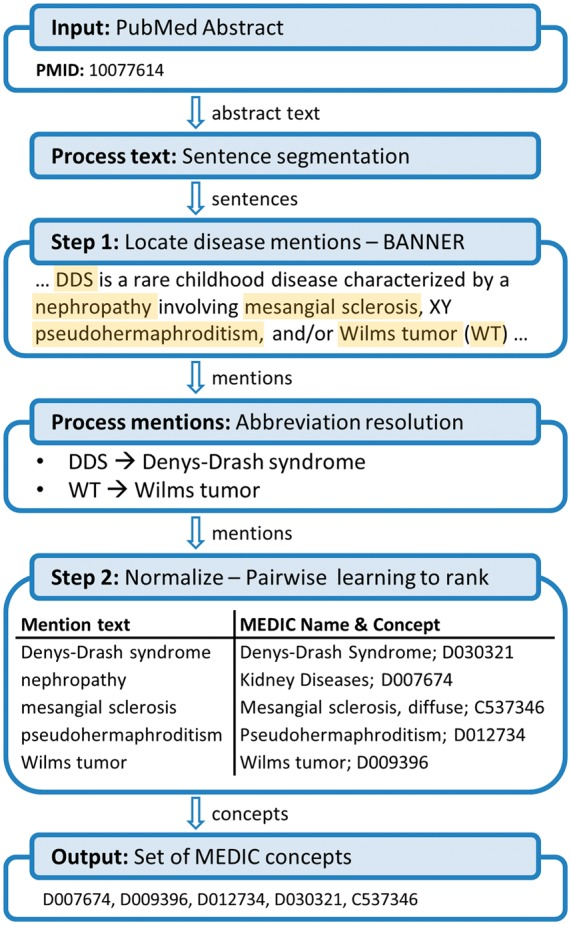
\includegraphics{Figures/dnorm.jpg}
    \rule{35em}{0.5pt}
  \caption[Overview of DNorm pipeline]{Overview of DNorm pipeline. The figure was taken from Leaman, Dogan and Lu, 2013 \citep{leaman2013dnorm}.}
  \label{fig:DNorm}
\end{figure}

The reason why we initially resorted to DNorm is because of its good performance with regard to precision, recall and F-measure \citep{leaman2013dnorm}. Also, the underlying tagging mechanism BANNER appeared to perform well in BioCreative benchmarks for tagging various biological entities, most notably gene names \citep{smith2008overview} \citep{leaman2008banner}. Trying to extend DNorm to support gene names recognition \textit{and normalization}, however, proved to be very difficult. We figured out that there was no publicly available compatible data set that we could use to train our model for gene normalization. Secondly, since the DNorm uses matrix to represents both the normalization and similarity model \citep{leaman2013dnorm}, creating matrix models for the whole set of proteins would have the program create a matrix with millions of row -- which wouldn't scale in normal cluster environment\footnote{The largest machine in our cluster provides 64 GB of memory in normal situation. A transition matrix with 100,000 starting and 100,000 target states with each transition represented as 64 bytes double precision entry will take \textit{at least} 8 * 100000 * 100000 $\approx$ 80 GB memory to initiate, \textit{conservatively}. We know that the number of the reviewed proteins alone is already beyond that at the time of writing of this thesis.}. Also, the fact that DNorm was optimized for disease names means that there is no guarantee that the resulting benchmark for protein names would be as good as disease tagging and normalization benchmark.

Later on, we switched to STRING Tagger. Unlike NER methods that are already mentioned in this chapter, our current NER Tagger relies on mapping between normalized entity names and their corresponding alternative names to annotate and normalize named entities within in the text. It checks whether a part of text closely resembles one or more elements in the mapping. It would then calculate the probability of the part of text being the instance of one of the entities (see more on Chapter \ref{Chapter4}). While there is no publication specifically dedicated for gene annotations, the underlying engine was used to tag and annotate taxonomic names in PubMed text (Pacifilis, et al., 2013 \citep{pafilis2013species}). Moreover, we used part of STRING database (Szklarczyk, et al., 2011 \citep{szklarczyk2011string}) as the dictionary between normalized entity names and its variation of names that would be used to identify named entities in text and at the same time normalize them.


%----------------------------------------------------------------------------------------
%	SECTION 5
%----------------------------------------------------------------------------------------

\section{Previous Works}

There are several publications and tools that attempt on similar goals as we do that have not been reviewed in previous section. While we are not aware of other project that realized end-to-end article search based on sequence, there are several (very successful) attempts on doing parts of it.

In the realm of \textbf{gene/protein names tagging and/or normalization}, there are various programs that are known to tag and normalize well such as GNAT (Hackenberg, et al. 2011 \citep{hakenberg2011gnat}), ABNER (Burr, 2015 \citep{settles2005abner}) and LINNEAUS (Gerner, et al. 2010 \citep{gerner2010linnaeus}). The latter was originally designed to detect and annotate taxonomy names within text but is now "intended for general-purpose dictionary matching software"\footnote{\href{http://linnaeus.sourceforge.net/}{\texttt{http://linnaeus.sourceforge.net/}}, accessed 8/19/2015}.

For searching for protein mentions within PubMed corpus we are for example aware of. Given a UniProtKB-ID, a user can search for the list of articles mentioning the protein. User could, for example, search articles that mention human tumor protein P53 (\texttt{P53\_HUMAN})\footnote{\href{http://www.uniprot.org/citationmapping/?query=uniprot:P04637}{\texttt{http://www.uniprot.org/citationmapping/?query=uniprot:P04637}}, accessed 24/08/2015}. We are unfortunately not aware how it was done (manually annotated or done using NLP methods) or whether it covers only parts of article that are visible within PubMed corpus or the whole article nor there exists any formal documentation/publication regarding the system.

\begin{figure}[htbp]
  \centering
    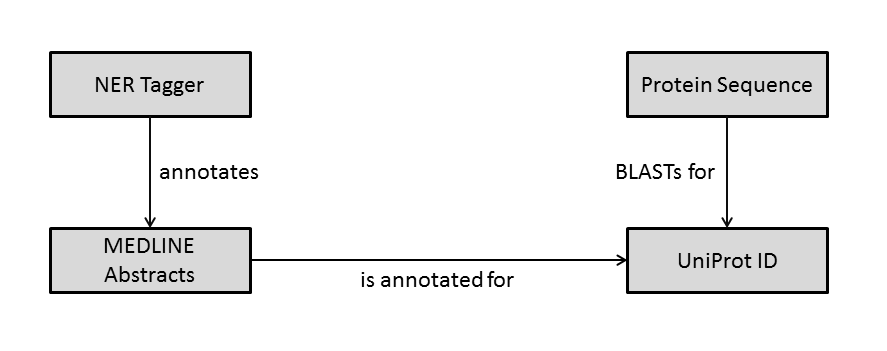
\includegraphics[width=6in]{Figures/component_graph.png}
    \rule{35em}{0.5pt}
  \caption[Schematic interaction between BLAST, UniProt, MEDLINE and NER Tagger]{Schematic interpretation on how the concepts of BLAST, UniProt, MEDLINE and NER are interrelated.}
  \label{fig:SchematicInteraction}
\end{figure}